% Overleaf: upload online_benchmark_comparison.pdf alongside this snippet.
% Requires \usepackage{graphicx} in the preamble.
\subsection{Computational Cost of Online Analysis}
\label{subsec:online_analysis_cost}

Online shock analysis was benchmarked against a scheduled solver baseline and
a workflow that retains full snapshots, analyzes them after integration, and
writes them as uncompressed files. Each workflow used the same wind-bubble
setup, a fixed injection radius of $0.0625$ in domain units, and 20 analysis
events over $0 \leq t \leq 0.20$. The baseline retained the same event-related
timestep boundaries. Measurements were performed on an NVIDIA H100 GPU using
JAX 0.6.2. Reported execution times are medians of three repetitions following
one warmup; compilation was measured separately and excluded.

At $64^3$ cells, online analysis increased the execution time from
$0.956\,\mathrm{s}$ to $1.424\,\mathrm{s}$, corresponding to an overhead of
$49.0\%$ relative to the scheduled solver. At $128^3$ cells, the corresponding
times were $12.728\,\mathrm{s}$ and $14.794\,\mathrm{s}$, giving an overhead
of $16.2\%$. Online execution was $26.8\%$ and $23.9\%$ faster than the
stored-snapshot workflow at the two resolutions, respectively. At $128^3$,
explicit compilation took $89.4\,\mathrm{s}$ for the online workflow and
$53.1\,\mathrm{s}$ for the stored-snapshot workflow; the execution-time
comparison therefore describes performance after compilation.

Output per trial decreased from $104.9\,\mathrm{MB}$ to
$36.1\,\mathrm{kB}$ at $64^3$, and from $838.9\,\mathrm{MB}$ to
$36.9\,\mathrm{kB}$ at $128^3$, where decimal storage units are used.
At $128^3$, the sampled GPU process-memory peak decreased from
$4912\,\mathrm{MiB}$ to $2858\,\mathrm{MiB}$, while peak host resident
memory increased from $1.61\,\mathrm{GB}$ to $1.89\,\mathrm{GB}$.
These memory measurements cover the whole worker lifetime, including
compilation and warmup; the sampled GPU values are lower bounds on the true
process-memory peaks.

For all three repetitions at both resolutions, online and offline histogram
counts matched exactly, scalar diagnostics agreed within relative and
absolute tolerances of $10^{-6}$ and $10^{-8}$, and the final simulation-state
hashes were identical across workflows. These results establish consistency
and reduced output storage for the tested configurations. They do not
establish physical convergence or general scaling behavior. Timings include
file writes without explicit synchronization to physical storage, and the
workflows ran in a fixed order on a shared machine.

\begin{figure}[htbp]
    \centering
    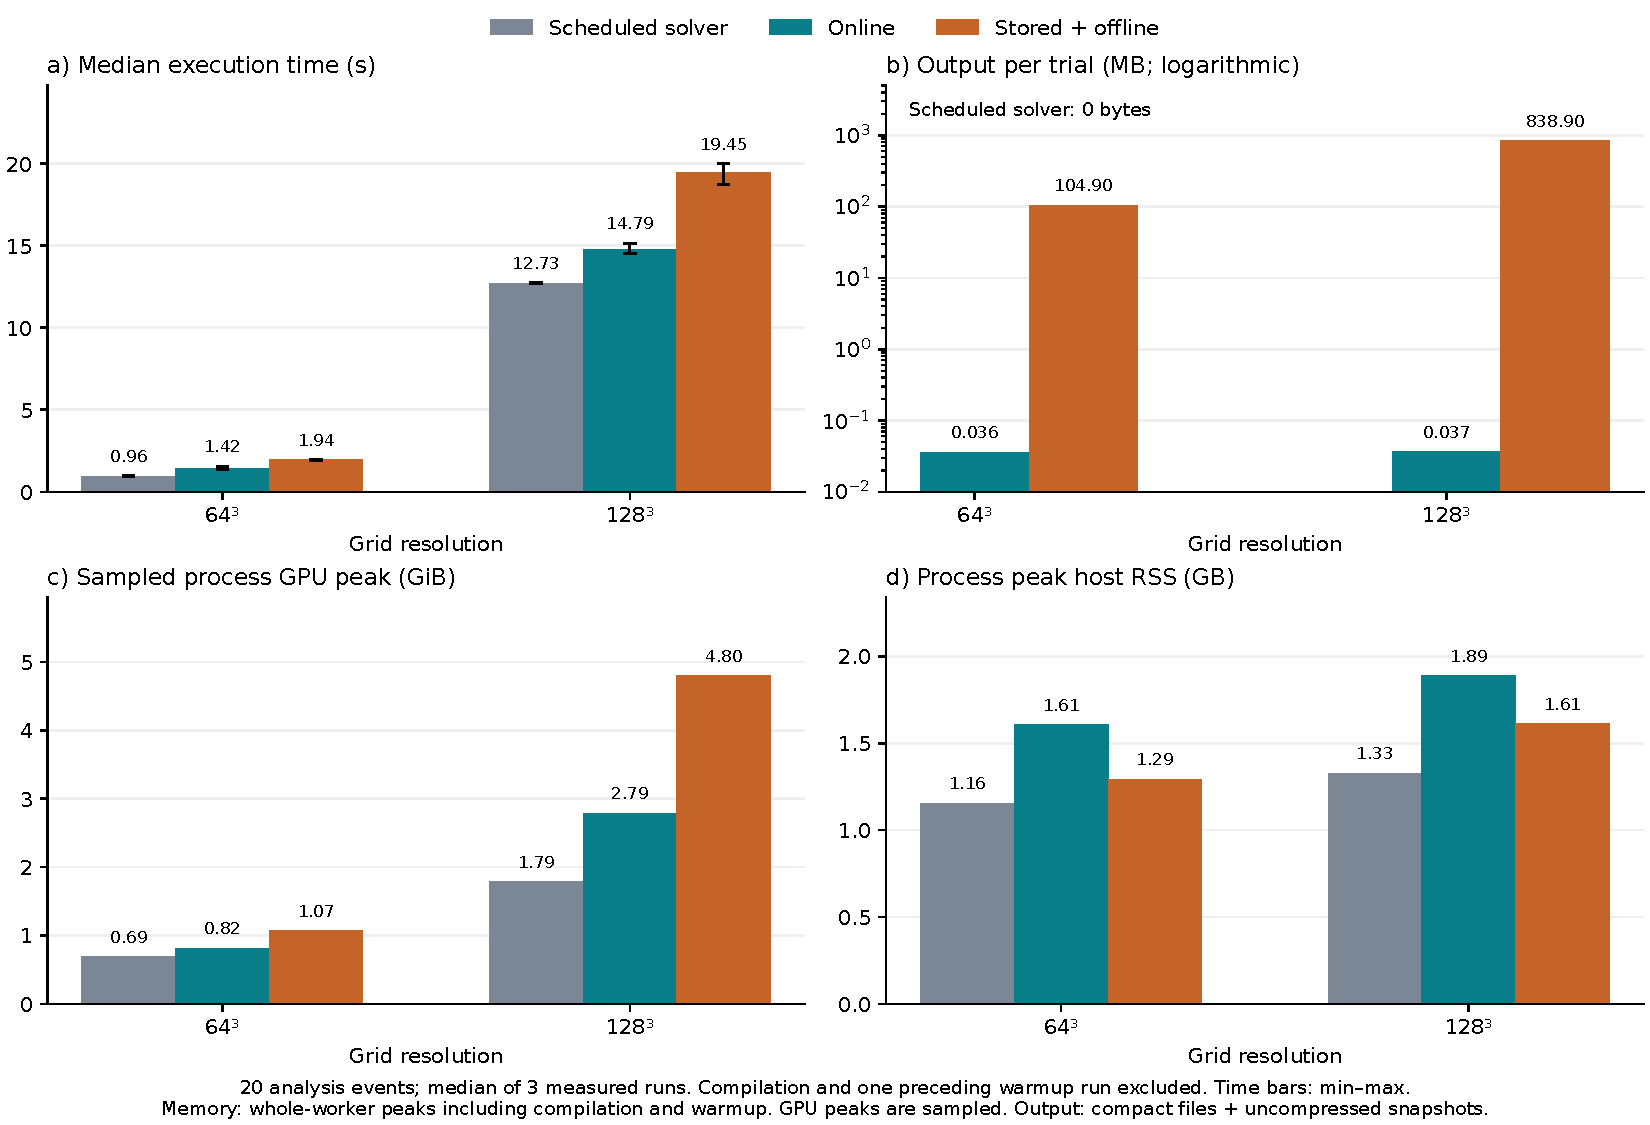
\includegraphics[width=\textwidth]{online_benchmark_comparison.pdf}
    \caption{Comparison of scheduled solver, online shock analysis, and
    stored-snapshot analysis at two grid resolutions. Execution times show
    medians and minimum--maximum ranges from three warmed trials and exclude
    compilation. Output includes compact diagnostics and, for the stored
    workflow, uncompressed snapshots. Memory values are whole-worker peaks;
    GPU memory was sampled. The solver baseline produces no diagnostic
    output and is omitted from the logarithmic output-size bars.}
    \label{fig:online_benchmark_comparison}
\end{figure}
